\section{Untersuchung von Mikrowellen}

	\subsection{Methoden}
		
		Der Aufbau dieses Versuches variiert für die verschiedenen Teilversuche.
		Für alle jedoch werden elektromagnetische Wellen (im Mikrowellenbereich) von einem Sender ausgesendet und von einem Empfänger aufgefangen und die dortige Intensität als Spannung, das Strahlprofil, gemessen.
		
		\subsubsection*{Strahlendivergenz}
		\begin{figure}[ht]
			\centering
			\includegraphics[width=0.6\textwidth]{bilder/Mikrowelle_1.png}
			\caption{Für den Versuch verwendete Materialien.\cite{WWU}}
			\label{fig:Aufbau1}	
		\end{figure}
		Zur Bestimmung der Strahlendivergenz wird wie in Abb. \ref{fig:Aufbau1} dargestellt, die Position des Empfängers über zwei Schienen verändert. 
		Jeweils eine horizontal und eine vertikal zu dem Sender liegende. 
		Damit lässt sich der virtuelle Quellfleck des Senders bestimmen.
		Die gemessenen Spannung sollen als Funktion des Ortes dargestellt werden. 
		
		\subsubsection*{Stehende Welle}
		\begin{figure}[ht]
			\centering
			\includegraphics[width=0.6\textwidth]{bilder/Mikrowelle_2.png}
			\caption{Für den Versuch verwendete Materialien.\cite{WWU}}
			\label{fig:Aufbau2}	
		\end{figure}
		Für die Erzeugung einer stehenden Welle wird eine Metallplatte gegenüber dem Sender platziert. 
		Dies ist in Abb. \ref{fig:Aufbau2} dargestellt.
		Der Empfänger liegt hierbei zwischen Sender und Metallplatte. 
		Bei stehenden Wellen ist an den Knotenpunkten für jede Zeit der gleiche Wert zu messen.
		Deswegen wird der Abstand zwischen Sender und Metallplatte so angepasst, dass sich solche Knotenpunkte mit dem Empfänger finden lassen.
		An der Metallplatte muss dafür ein Knoten liegen und der Abstand zweier Knoten entspricht einer halben Wellenlänge.
		Diese lässt sich also über das Messen zweier Knotenpunkte bestimmen.
		
		\subsubsection*{Brechungsindexbestimmung}
		\begin{figure}[ht]
			\centering
			\includegraphics[width=0.6\textwidth]{bilder/Mikrowelle_3.png}
			\caption{Für den Versuch verwendete Materialien.\cite{WWU}}
			\label{fig:Aufbau3}	
		\end{figure}
		Danach soll ein PVC-Halbzylinder untersucht werden. 
		Dieser befindet sich wie in Abb. \ref{fig:Aufbau3} zu sehen fixiert über einer mit einer Schiene verbundenen drehbaren Platte auf der Winkel eingezeichnet sind.
		So lässt sich nach dem Snellius'schen Brechungsgesetz
		\begin{equation}
			n_1 \sin{\phi_1} = n_2 \sin{\phi_2}
		\end{equation}
		der Brechungsindex $n_\text{PVC}$ des Halbzylinders bestimmen. 
		Die benötigten Winkel dafür lassen sich der drehbaren Platte entnehmen und der Brechungsindex von Luft $n_\text{Luft}$ entspricht in etwa 1.
		
		\subsubsection*{Frustrierte Totalreflexion}
		\begin{figure}[ht]
			\centering
			\includegraphics[width=0.6\textwidth]{bilder/Mikrowelle_4.png}
			\caption{Für den Versuch verwendete Materialien.\cite{WWU}}
			\label{fig:Aufbau4}	
		\end{figure}
		Für den Winkel $\phi\text{PVC}$, bei dem $\phi\text{Luft}$ bei \SI{90}{\degree} liegt, tritt das Phänomen der Totalreflexion auf, was bedeutet, dass die elektromagnetische Welle keinen transmittierten Teil mehr besitzt, sondern vollständig an der Grenzfläche reflektiert wird. 
		Da die elektromagnetische Welle jedoch eine gewisse "Breite" besitzt, breitet diese sich nahe der Grenzfläche, wenn auch exponentiell abfallend in dem angrenzenden Medium aus.
		Diesen Teil nennt man evaneszente Welle.
		Bringt man ein weiteres Medium mit größerem Brechungsindex näher, so wird diese evaneszente Welle in diesem Medium "zurückgebrochen" und breitet sich darin weiter aus.
		Diese "frustrierte" Totalreflexion soll für diesen Versuch mit einem zweiten PVC-Halbzylinder veranschaulicht und gemessen werden. 
		Dazu Abb. \ref{fig:Aufbau4}.
		Die gemessene Intensität an dem Empfänger soll zudem in Abhängigkeit des Abstands der Zylinder aufgetragen werden.		
		
		\subsubsection*{Bragg'sche Reflexion}
		\begin{figure}[ht]
			\centering
			\includegraphics[width=0.6\textwidth]{bilder/Mikrowelle_5.png}
			\caption{Für den Versuch verwendete Materialien.\cite{WWU}}
			\label{fig:Aufbau5}	
		\end{figure}
		Zuletzt soll ein Metallkugelgitter in einem Schaumstoffquader untersucht werden (vgl. Abb. \ref{fig:Aufbau5}). 
		Dieser liegt auf der drehbaren Platte und zwar so, dass bei dem Drehen der Schiene der Quader so mitgedreht wird, dass für Sender und Empfänger immer Einfallswinkel $\alpha$ = Ausfallswinkel gilt.
		Über die Bragg'sche Reflexion
		\begin{equation}
			2d\sin{\alpha} = n\lambda
		\end{equation}
		lässt sich der Abstand zwischen den Gitterebenen $d$ bestimmen.
		Zur Veranschaulichung dient Abb. \ref{fig:bragg}.
		\begin{figure}[ht]
			\centering
			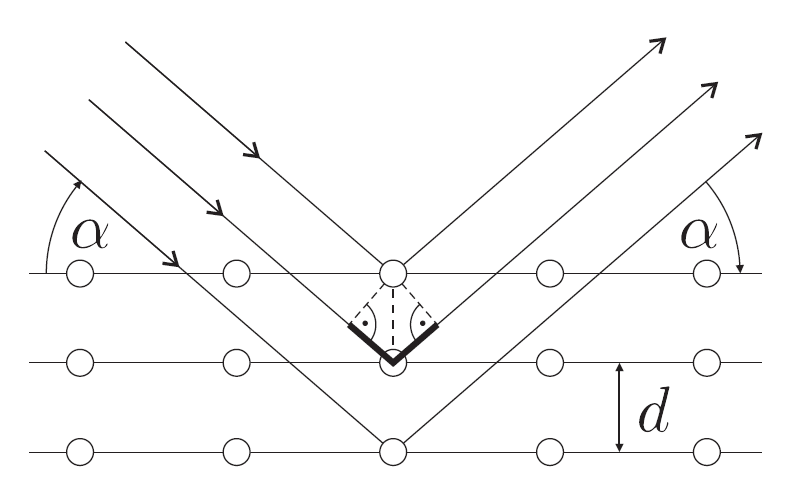
\includegraphics[width=0.6\textwidth]{bilder/Bragg.png}
			\caption{Für den Versuch verwendete Materialien.\cite{WWU}}
			\label{fig:bragg}	
		\end{figure}
		Der sogenannte Glanzwinkel $\alpha$ wird durch Drehung der Platte und Intensitätsmessung an dem Empfänger festgelegt und die zuvor bestimmte Wellenlänge zur Bestimmung des Gitterabstandes $d$ verwendet. 
		
	\subsection{Durchführung}
	
		% TODO
	
	\subsection{Datenanalyse}
		
		% TODO
	
	\subsection{Diskussion}
	
		% TODO